\documentclass[twocolumn,amsmath,longbibliography,amssymb,superscriptaddress]{revtex4-1}
\usepackage[pdftex]{graphics}
\usepackage{graphicx}
\graphicspath{{figures/}}
\usepackage{hyperref}
\usepackage{xcolor}
\usepackage{physics}
\usepackage{subfig}
\usepackage{bm}
\usepackage{caption}
\usepackage{amsmath} 

\newcommand{\carlos}[1]{{\color{red} #1}}
\newcommand{\maria}[1]{{\color{blue} #1}}
\newcommand{\mariac}[1]{{\it\color{cyan}#1}}

	
\begin{document}
		
\title{On the relation of the entanglement spectrum to the Zak-phase}
\author{Carlos Ortega Taberner}
\affiliation{Department of Physics, Stockholm University, AlbaNova University Center, SE-106 91 Stockholm, Sweden}
\affiliation{Nordita, KTH Royal Institute of Technology and Stockholm University, SE-106 91 Stockholm, Sweden}

\author{Maria Hermanns}
\affiliation{Department of Physics, Stockholm University, AlbaNova University Center, SE-106 91 Stockholm, Sweden}
\affiliation{Nordita, KTH Royal Institute of Technology and Stockholm University, SE-106 91 Stockholm, Sweden}
\date{\today}
		
\maketitle
	


\section{Introduction}
Topological phases of matter have attracted a lot of attention during the last decades, not the least because a large variety of relevant systems have been realized experimentally. 
The early focus was mainly on \emph{topologically ordered} systems \cite{wenbook}, where interaction effects are crucial for stabilizing the phase. 
The most notable examples are the fractional quantum Hall effect~\cite{Tsui1982} and quantum spin liquids~\cite{Balents2010spin}. 
However, since 2005~\cite{kane2005quantum, roy2009topological} the focus has shifted to non-interacting topological phases, which can be characterized in terms of topological invariants~\cite{ryu2010topological}. 
Symmetries are often necessary to protect these topological phases, and determine which distinct topological phases can be realized for a given dimensionality. 

There are few tools to identify topological phases. 
A very efficient one is the entanglement entropy~\cite{Kitaev2006topological, Levin2006detecting}, which allows one to identify the total quantum dimension of the underlying topological quantum field theory. 
As such, the entanglement entropy can only be used for interacting systems. 
Its main drawback is the fact that it can only provide one of the pertinent quantum numbers that characterizes the system, and is, thus,  not able to uniquely determine the topologically ordered phase at hand. 
In addition, it requires a careful scaling analysis, which can be challenging for strongly correlated systems. 
Another, closely related tool, is the entanglement spectrum (ES), originally introduced for fractional quantum Hall systems~\cite{Li2008entanglement}. 
It was conjectured to provide information about the edge spectrum, which was later shown to be a general feature of ground states with an effective topological quantum field theory description~\cite{Qi2012general}. 
It also proved to be an effective tool for fractional Chern insulators~\cite{Regnault2011fractional} and certain quantum spin liquids~\cite{yao2010entanglement}. \mariac{Others?}

Generically, any of the proposed tools provides some information about the phase naturally, while others seem inaccessible. 
It is not known, whether there exists a method to obtain the full topological data from the ground state. 
For the simplest quantum Hall states, the Laughlin states,  it was shown that the ES does, in fact, contain the full information about the topological phase~\cite{hermanns2011haldane}.
However, it is far from clear if this holds for more complicated, in particular nonabelian, states as well.  

Here, we address a much simpler question: what information can be extracted from the ES of \emph{non-interacting} systems?
The latter can be computed very efficiently, using methods developed by Peschel and others~\cite{Peschel2003}. 
It was subsequently shown for topological insulators/superconductors that the ES for (gapped) periodic systems is equivalent to the flat-band energy spectrum of the corresponding system with open boundaries~\cite{Fidkowski2010entanglement}. 
The same correspondence was also found for closely related gapless systems~\cite{Matern2018entanglement}
However, even for non-interacting systems, it is unclear which information (beyond the  `edge' spectrum) is encoded in the spectrum. 

In this manuscript, we show that the information about the Zak phase can be completely recovered from the entanglement spectrum and provide a simple formula to do so. 
The relation between the entanglement spectrum and various topological invariants has already been studied in the literature. 
In Ref.~\cite{Zaletel2014}, the authors show that the Zak phase can be computed from the Schmidt decomposition of a translation invariant, infinite chain. 
This demonstrates that there should be a direct relation between the single-particle entanglement energies and the Zak phase, although deriving that relation turned out to be non-trivial. 
An added benefit of our approach is that it can be generalized to systems that are not translationally invariant in a numerically efficient way. 
A particular limit of our result for homogeneous systems~\ref{eqplusminus} was derived by Ryu and Hatsugai for a fully dimerized SSH chain~\cite{Ryu2006}. 
The similarity between the behavior of the Zak phase and the 'virtual edge modes' in the entanglement spectrum of a Chern insulator, which was observed in Ref.~\cite{Huang2012,Huang2012-2}, can also be explained by our results. 


\emph{Outline of the paper}: In section II we introduce the model used throughout the paper and we discuss its phase diagram. In section III we introduce the Zak phase and the entanglement spectrum and set up the notation that will be used. In section IV and V we show our results for homogeneous and inhomogeneous systems, respectively. In section VI we will discuss how our results also generalize to the case of models with pairing terms and finally in section VII we present the conclusions and possible outlook.

% - % - % - % - % - % - % - % - % - % - % - % - % - % - % - % - % - % - % - % 
\section{Model.}
To showcase our results we consider as a starting point the model in the BDI class used in reference~\cite{Song2014}. 
This is a very simple model which nevertheless supports a rich phase diagram containing topological phases with winding numbers up to $\nu =2$. 
In order to show that our results are not limited to any symmetry class~\cite{ryu2010topological}, we also include two symmetry breaking terms. 
The Hamiltonian is  given by
\begin{align}
H =& \sum_{i\alpha,j\beta} c_{i\alpha}^\dagger H_{ij,\alpha \beta} c_{j\beta} \\
H_{ij} =& (m \sigma_x + \kappa \sigma_z)\delta_{ij}  + \frac{1}{2i}\kappa'\sigma_z (\delta_{i-j,1}-\delta_{i-j,-1})\nonumber\\
&+ \frac{1}{2} t \left[(\sigma_x + i \sigma_y)\delta_{i,j+1} + (\sigma_x - i \sigma_y) \delta_{i,j-1} \right] \nonumber\\
&+  \frac{1}{2} t' \left[(\sigma_x + i \sigma_y)\delta_{i,j+2} + (\sigma_x - i \sigma_y) \delta_{i,j-2} \right],
\label{bdi_model}
\end{align}
with the corresponding Bloch Hamiltonian being
\begin{align}
H(k)=&\mqty( \kappa + \kappa' \sin(k) & t' e^{i2k} + t e^{ik}+m \nonumber\\t' e^{-i2k} + t e^{-ik}+m & -\kappa-\kappa' \sin(k)  )\nonumber \\
=& (t' \cos(2k)+t\cos(k)+m)\sigma_x \\
&+ (-t' \sin(2k)-t\sin(k))\sigma_y + (\kappa+\kappa'\sin(k)) \sigma_z.\nonumber
\end{align}

For $\kappa = \kappa' = 0$ this Hamiltonian is in the BDI class, i.e. it has time-reversal ($T$), particle-hole ($C$), and chiral symmetry ($S$):
\begin{alignat}{2}
&T = \mathcal{K} ; \quad &&T H(-k) T^{-1} = H(k) \nonumber\\
&C = \sigma_z\mathcal{K} ; \quad &&C H(-k) C^{-1} = -H(k) \nonumber\\
&S = \sigma_z ; \quad &&S H(k)S^{-1} = -H(k) .
\end{alignat}
Using the results of Ref.~\cite{Song2014}, the corresponding phase diagram can be calculated and is shown in Fig.\ref{fig:bdi_phase_diagram} for $t=1$. 
\begin{figure}[t]
	\centering
	\makebox[0pt]{
	\subfloat[$t = 1,\kappa =\kappa'=0$]{
	  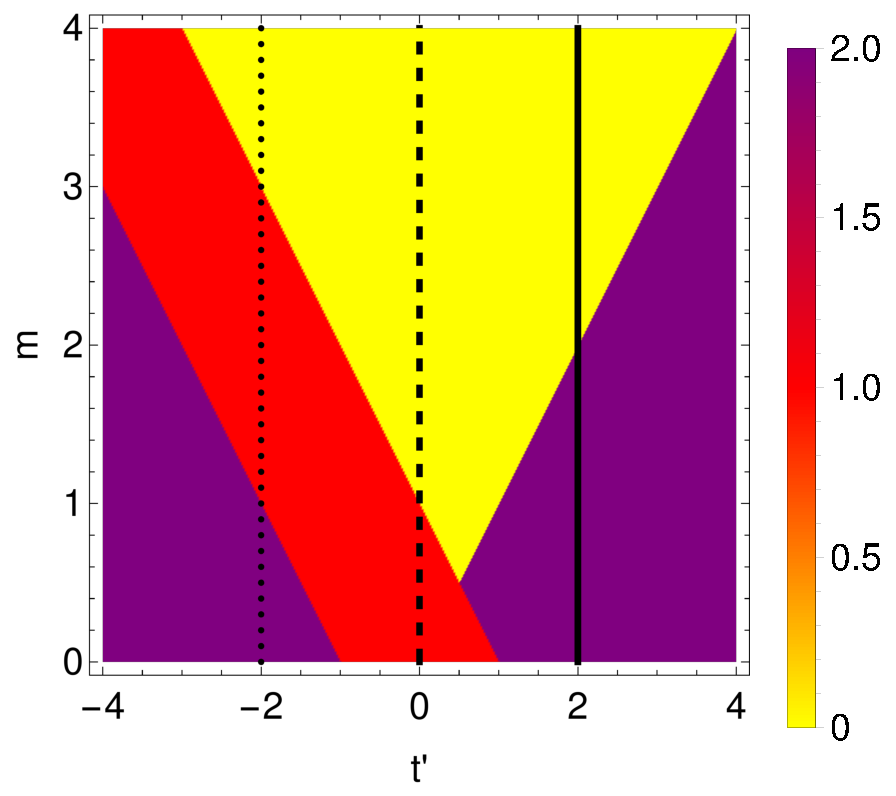
\includegraphics[width=45mm]{phase_diagram2.pdf}
	}}\hspace{0mm}
\caption{\mariac{ Get rid of (a).}Phase diagram for the system in the $BDI$ class showing the winding number of each region.}
\label{fig:bdi_phase_diagram}
\end{figure}
The BDI class  is characterized by a $\mathbb{Z}$ invariant, the winding number,  in one spatial dimension.
When imposing open boundary conditions on the system, the number of symmetry-protected zero energy edge modes is equal to the winding number. 
The behavior of the  edge modes  is  shown in Fig.~\ref{fig:zero_E_modes}, using the dotted path ($t=1,t'=-2$) marked in the phase diagram. 
Subfigure (a) shows the edge spectrum in the BDI class, with 4 (resp. 2) symmetry-protected zero modes for winding number 2 (1). 
%We also a cut through the three phases (dotted line in the phase diagram) for different values of $\kappa,\kappa'$.  

For $\kappa' \neq 0$ only particle-hole symmetry $C$ is preserved and the system belongs to symmetry class $D$. 
In one spatial dimension, the latter is characterized by a $\mathbb{Z}_2$ invariant.  
Consequently, adding such a term causes the zero modes in the $\nu=2$ phase to split  pairwise and the $\nu = 2$ and $\nu=0$ phases become equivalent. 
This is shown in subfigure (c), where one clearly sees that the zero modes below $m=1$ are split. 

For $\kappa \neq 0$ only time-reversal $T$ is preserved and the system is in the AI class. 
In one dimensions, this class is trivial and, thus,  all zero-energy modes split. 
With both $\kappa \neq 0$ and $\kappa' \neq0$ the system has no symmetry, thus belonging to the $A$ class.  
Also this symmetry class is topologically trivial in one dimension. 
Subfigures (b) and (d) show the edge spectrum for class AI and A, respectively. In both cases, the edge modes are split from zero for all values of $m$.


%
%In subfigure (b) and (d), where the system is in a topologically trivial phase, all edge modes are gapped. 
%Subfigure (c) shows the edge spectrum of the system being in class D, where the $\nu=2 $ phase becomes trivial. 
%Consequently, symmetry-protected zero modes only exist for $1<m<2.5$\mariac{?} (corresponding to $\nu=1$ for $\kappa'=0$) , whereas the modes are split for $m<1$ (corresponding to $\nu=2$ for $\kappa'=0$).

\begin{figure}[h!]
\centering
%\makebox[0pt]{
%\subfloat[$t = 1,\kappa =\kappa'=0$]{
%  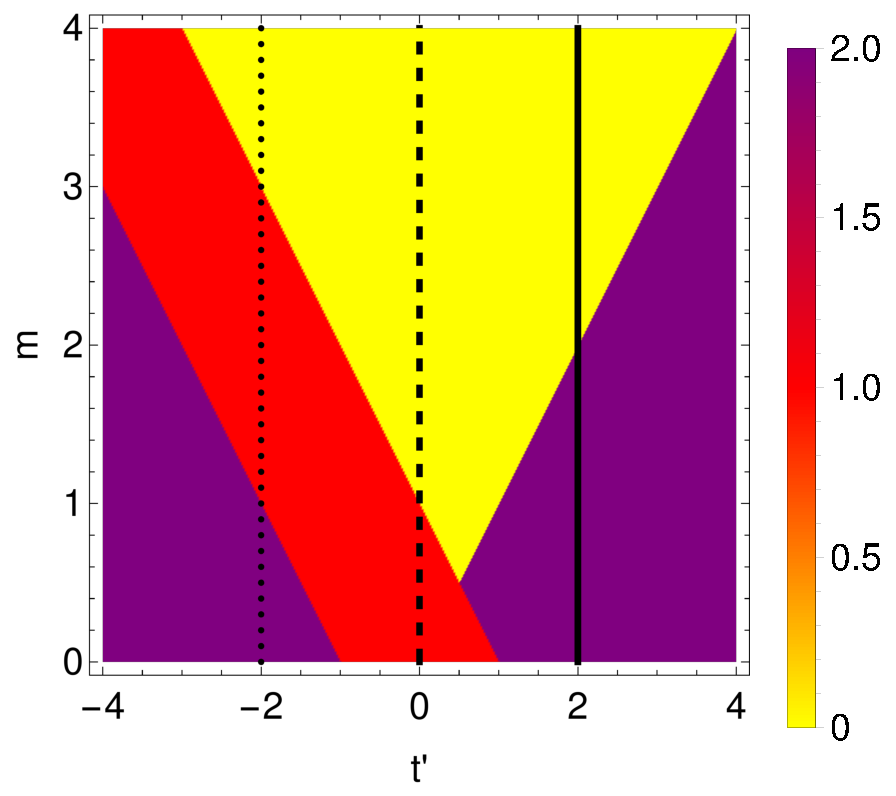
\includegraphics[width=45mm]{phase_diagram2.pdf}
%}}\hspace{0mm}

\makebox[0pt]{
\subfloat[$\kappa =\kappa'=0$]{
  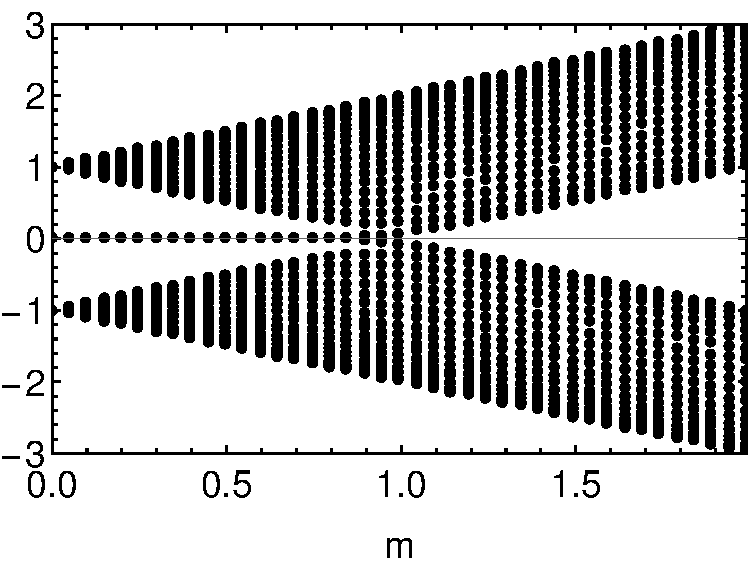
\includegraphics[width=35mm]{1_a.pdf}
}
\subfloat[$\kappa = 0.3, \kappa'=0$]{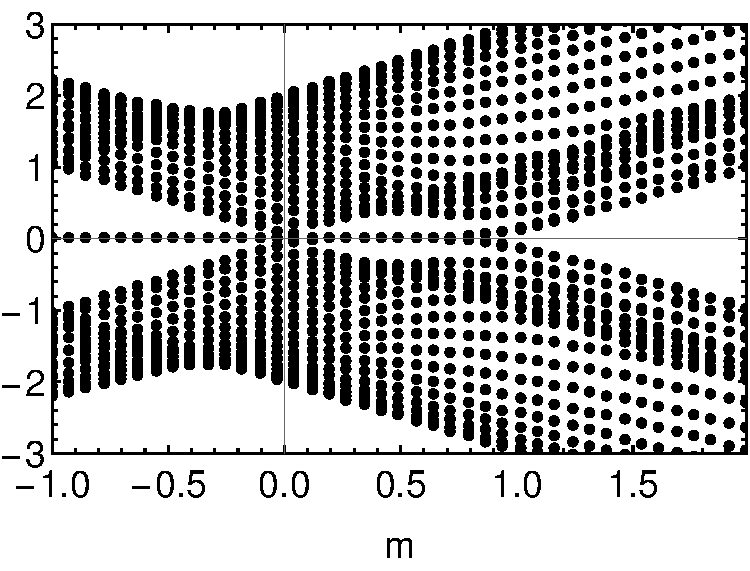
\includegraphics[width=35mm]{1_b.pdf}
}
}\hspace{0mm}

\makebox[0pt]{
\subfloat[$\kappa = 0,\kappa'=0.3$]{
  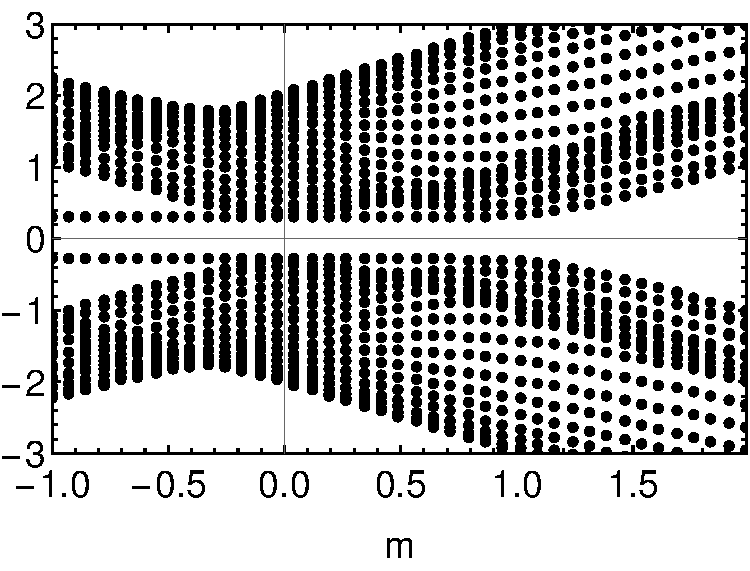
\includegraphics[width=35mm]{1_c.pdf}
}
\subfloat[$\kappa = 0.3,\kappa'=0.3$]{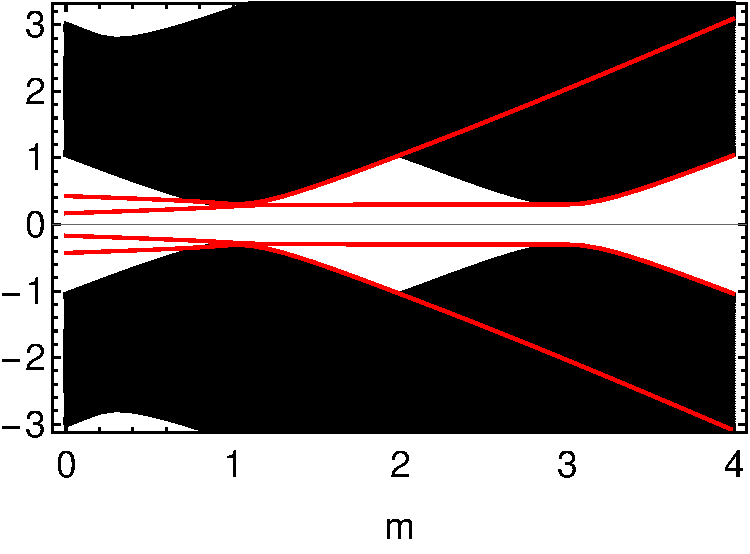
\includegraphics[width=35mm]{1_d.pdf}
}
}
\caption{\mariac{increase system size and colorcode edge modes.}Edge spectrum along the dotted path (i.e. $t=1,t'=-2$) of Fig.~\ref{fig:bdi_phase_diagram} for different values of $\kappa$ and $\kappa'$.\mariac{note on numerical system size}}
\label{fig:zero_E_modes}
\end{figure}

% - % - % - % - % - % - % - % - % - % - % - % - % - % - % - % - % - % - % - % - % - % - % - % - % - % - % - % - % - % - % - % - % - % - % - % - % - % 
\section{Zak phase and entanglement spectrum}
In this section, we review some relevant information about firstly the Zak phase and secondly the entanglement spectrum in non-interacting systems. 
We consider a generic, quadratic Hamiltonian in one dimension
\begin{equation}\label{eq:quadr_Ham}
\mathcal{H} = \sum_{ij,\alpha\beta} c_{i\alpha}^\dagger H_{ij,\alpha \beta}c_{j\beta}.
\end{equation}
We can obtain the single-particle eigenstates as
\begin{align}
\sum_{j\beta}H_{ij,\alpha\beta} u^{p\mu}_{j\beta} = E_{p\mu} u_{i\alpha}^{p\mu},
\end{align}
where $[U]_{j\beta,p\mu} = u^{p\mu}_{j\beta}$ is the unitary matrix that diagonalizes $H$. 

In translational invariant systems the Zak phase is defined as the Berry phase acquired by a state $\ket{u_k}$ as it winds around the Brillouin zone,
\begin{equation}
\gamma = \int_{-\pi}^\pi dk \, \bra{u_k}\partial_k \ket{u_k} \, {\rm mod}\, 2\pi.
\end{equation}
The Zak phase is equal to $\pi$ times the parity of the winding number, and it is also related to the polarization \cite{Resta1997}. Since the latter has a position space formulation we will use  it in all calculations below to compute the Zak phase. 

The polarization can be obtained as the many-body average of the position operator, but the latter has to be regularized for periodic boundary conditions \cite{Resta1997}. 
We can define a position operator for PBC as
\begin{equation}
\hat{X}_{\rm PBC} = e^{-i\frac{2\pi}{L}\hat{X}},
\end{equation}
where $\hat{X}$ is the sum of all the single-particle position operators. 

We can now consider then the many-body average of the position operator over the ground state, defined as
\begin{align}
\expval{\hat{X}_{\rm PBC}}_0 \equiv -\frac{L}{2\pi} \rm{ Im }\ln\bra{\Psi_0}\hat{X}_{\rm PBC}\ket{\Psi_0},
\end{align}
%\carlos{This is the notation used in the Resta paper, but I'm not sure if it's confusing.}
where $\ket{\Psi_0}$ is the many-body ground state. 
Using that the ground state is a Slater determinant of the occupied single-particle eigenstates, $\ket{u^{p\mu}}$, it can be rewritten as~\cite{Resta1997}
\begin{align}
\expval{\hat{X}_{\rm PBC}}_0 = -\frac{L}{2\pi} \rm{Im }\ln \, {\rm det }\!' \, S,
\end{align}
where the matrix $S$ is given by
\begin{equation}
S_{p\mu,q\nu} = \sum_{j\alpha} u^{p\mu\, \ast}_{j \alpha} e^{-i\frac{2\pi}{L}j}u^{q\nu}_{j \alpha}
\end{equation}
and  ${\rm det }\!' $ indicates that the determinant is restricted to the space of \emph{occupied} single-particle states. 
The Zak phase can then be obtained as
\begin{equation}
\gamma = \expval{\hat{X}_{\rm PBC}}_0\frac{2\pi}{L} + \frac{1}{2}.
\end{equation}
\carlos{There is an extra 1/2 factor compared to Restas's formula which I don't know where it is coming from.}

Let us now proceed to discuss the entanglement spectrum. 
An important quantity is the correlation matrix, which in position space is defined by
\begin{align}
C_{ij}^{\alpha \beta} = \expval{c_{i\alpha}^\dagger c_{j\beta}}.
\end{align}
Using the results of appendix~\ref{app:CM}, it  can be written  as
\begin{align}\label{eq:corr_mat2}
C_{ij}^{\alpha \beta} =& \frac{1}{2}\left[I - H/ (H^2)^{-1/2} \right]_{ij, \alpha \beta}.
\end{align}
This form is particularly useful for all our subsequent calculations, since it does not rely on translation symmetry. 

In this manuscript, we are mainly interested in the spectrum of the correlation matrix, when restricted to a spatial sub-region $A$ (its complement will be denoted by $B$ in the following). 
Following Ref.s~\cite{Huang2012,Huang2012-2}, we refer to this spectrum as the entanglement occupancy spectrum (EOS). 
The resulting eigenvalues  are denoted by $\xi_j$. 
%We will differentiate between two types of eigenvalues: those (exponentially) close to $\xi_j=0 (1)$ correspond to ``bulk'' states, by which we mean that the corresponding eigenstates lie (up to exponentially small corrections) in  $A$ ($B$). 
%Values $0<\xi_{l,r}<1$ indicate states that are located at the virtual boundaries -- labeled `left' and `right' in the following-- between $A$ and $B$~\cite{Peschel2008}. 
%There is, of course, an ambiguity here on dividing eigenstates of the EOS into ``bulk'' and ``edge'' states and `how close' the eigenvalue has to be to $0,1$ in order to qualify as a bulk state. 
%XXXX
Topological phases are characterized by (symmetry-protected) zero-energy modes in the edge spectrum and $\xi=\frac 1 2$ modes in the OES~\cite{Fidkowski2010entanglement}.
 

The EOS is in one-to-one correspondence to the entanglement spectrum (ES). 
Following Ref.~\cite{Peschel2008}, one can write the  reduced density matrix as 
\begin{align}\label{eq:red_dens_mat}
\rho_A&=\mathcal{K} \exp(-\mathcal H),
\end{align}
where $\mathcal{K}$ is a normalization constant and $\mathcal{H}$ is a quadratic Hamiltonian, referred to as entanglement Hamiltonian. 
The eigenvalues $\epsilon_j$ of $\mathcal{H}$, referred to as entanglement energies,  are related to the EOS by 
\begin{align}\label{eq:xi_eps}
\xi_j &=\left(e^{\epsilon_j}+1\right)^{-1}, 
\end{align}
the corresponding eigenstates are the same. 
Eq.~\eqref{eq:xi_eps} implies that the full information of the \emph{many-particle} ES is contained in the single-particle spectrum of the reduced correlation matrix. 
The latter is much simpler to interpret. 
Consequently, we will focus on the EOS in the remainder of the manuscript and only mention the ES when necessary. 
%The single-particle entanglement spectrum (ES) is then obtained as the spectrum of the subsystem correlation function obtained after bisecting the system into two equal parts. 

%In the ES we can differentiate between two types of eigenvalues, which we denote by $\xi$. The ones at $\xi_b = 0,1$ correspond to bulk states while for the ones in between, $0<\xi_{l,r}<1$, we find their correspondent eigenstate localized in either the left, $\xi_l$, or right, $\xi_r$, virtual edge \cite{Peschel2008}. 
%\mariac{introduce entanglement energy, relation between C and energies}


A few comments are needed regarding  bipartition. 
In the following sections, we show how the Zak phase can be recovered from the EOS.
We also give a simple formula that is identical to the Zak phase in the thermodyamic limit.  
However, for a generic, finite size system, there will be finite-size discrepancies between our formula and the Zak phase.
In order to reduce these, we are going to choose $A$ as half the system in the remainder of the manuscript.
The results (in the thermodynamic limit) do not depend on this choice. 
% - % - % - % - % - % - % - % - % - % - % - % - % - % - % - % - % - % - % - % - % - % - % - % - % - % - % - % - % - % - % - % - % - % - % - % - % - % 
\section{Homogeneous system}

Let us first review previous results on the relation between the entanglement spectrum and the Zak phase. 
For symmetry-protected topological systems in one dimension, the quantized Zak phase is zero whenever there is an even number  of eigenvalues per edge at $\xi = 1/2$, and $\pi$ when the number is odd~\cite{Peschel2008}. 
Ryu and Hatsugai considered the fully dimerized SSH chain with broken chiral symmetry~\cite{Ryu2006}.  
This model is rather special in that there is only a single pair of eigenvalues in the EOS that is not identical to $0$ or $1$. 
In fact, the authors could show that the value of this `midgap state' is identical to the Zak phase divided by $2\pi$. 
Their result is a particular limit of Eq.~\eqref{eqplusminus}. 
%
%Beyond symmetry protected systems, there was observed that in the fully dimerized SSH chain, with only a single mode present in the ES, the Zak phase is equal to the midgap eigenvalue \cite{Ryu2006}. 
Huang and Arovas considered a two-dimensional chern insulator and noted that the Zak phase qualitatively follows the `virtual edge mode' that connects the EOS values at 0 to those at 1~\cite{Huang2012,Huang2012-2}. 
Interpreting this as a one-dimensional system with a parameter, we can explain this behavior by Eq.~\eqref{eqplusminus}, noting that there is a single pair of eigenvalues that dominates the sum. 
Note that the observation of Ref.s~\cite{Huang2012,Huang2012-2} is particular to a system with Chern number 0 or $\pm 1$, and it generically fails for systems with higher Chern numbers.
In the latter case, there are several terms in Eq.~\eqref{eqplusminus} with comparably large contributions. 
%For cases with more edge modes present in the ES it has been shown that the Zak phase follows the midgap eigenvalues qualitatively \cite{Huang2012,Huang2012-2}. 


\subsubsection{Systems with equidistant entanglement energies}
\mariac{add scaling plot for $\chi$ versus $\gamma/(2\pi)$. }
We first discuss systems, for which the entanglement energies of a \emph{single} virtual edge are equidistant. 
This is a common feature for e.g. nearest neighbor hopping models\mariac{ref to Peschel}, such as the SSH chain, and applies to the Hamiltonian~\eqref{bdi_model} when $t'=0$. 
In this case, one can obtain the Zak phase in a very simple fashion: We reorder the eigenvalues of the ES by magnitude, $\xi_1 < \xi_2 < ...$, and compute
\begin{equation}
\chi = \frac{1}{2}\left(\sum_j (-1)^j \xi_j+N_A\right) \, {\rm mod} \, 1,
\label{eqplusminus}
\end{equation}
where $N_A$ is the number of electrons in the ground state in region A. 
In the thermodynamic limit, $\chi$ becomes identical to the Zak phase divided by $2\pi$:
\begin{equation}
\lim_{L \rightarrow \infty} \frac{\gamma}{2\pi} = \lim_{L \rightarrow \infty} \chi.
\end{equation}

In the case where there is only one eigenvalue per edge that is $\neq 0,1$ in  the EOS, like in the fully dimerized limit of the SSH chain, we recover the equality between the midgap eigenvalue and the Zak phase~\cite{Ryu2006}. 

In Fig.~\ref{huang} we show  the EOS along the dashed cut in the phase diagram of Fig.~\ref{fig:bdi_phase_diagram}. 
Along this line, our model is equivalent to an SSH chain. 
In the presence of chiral and translation symmetry, all eigenvalues of the EOS are doubly degenerate --- one eigenvalue from each edge. 
The difference of $\pi$ between the trivial and topological regime originates from the rearrangement of a few dominant eigenvalues in the EOS. 
In the topological regime, there are a pair of eigenvalues at $\xi=1/2$, while the rest are close to $0$ and $1$. 
At the phase transition, the two $\xi=1/2$ modes mix with one mode coming from $1$ and $0$ respectively, leading to a pair of modes close to $0$ and $1$, see Fig.~\ref{huang}(a). 
Consequently, there is one less mode at $\xi=1$, which yields a difference of $\pi$ in the Zak phase. 
Note that the full sum~\eqref{eqplusminus}  evaluates to zero in the trivial regime, up to finite-size corrections, despite the presence of modes with entanglement occupancy $0<\xi<1$. 

When breaking chiral symmetry, the EOS will no longer be doubly degenerate. 
For small $m$, there are two dominant midgap eigenvalues, and the Zak phase follows the lower of them very closely, see Fig.~\ref{huang}(b).
When this midgap eigenvalue approaches  0, the contribution from the other modes becomes more relevant and the Zak phase starts to deviate from the midgap eigenvalue, \mariac{see inset}.
\begin{figure}[h!]
\centering
\makebox[0pt]{
\subfloat[$t = 1,t'=0$, \, \,$\kappa =\kappa'=0$]{
  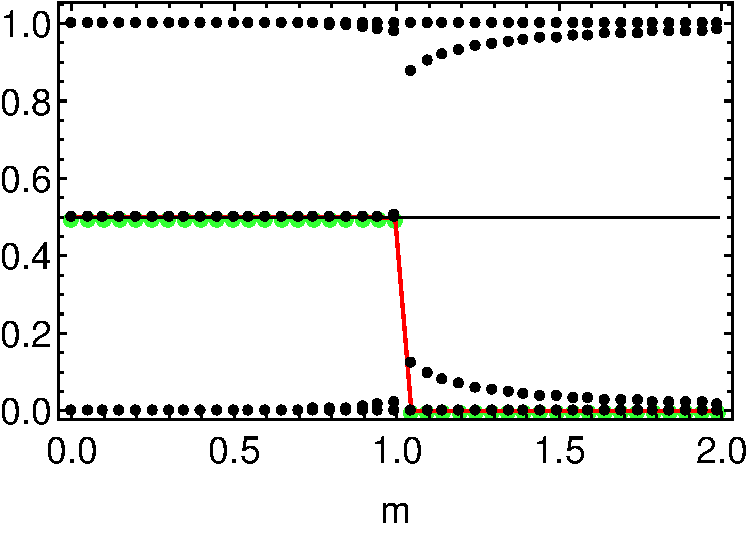
\includegraphics[width=35mm]{2_a.pdf}
}
\subfloat[$t=1,t'=0$, $\kappa = 0.3, \kappa'=0$]{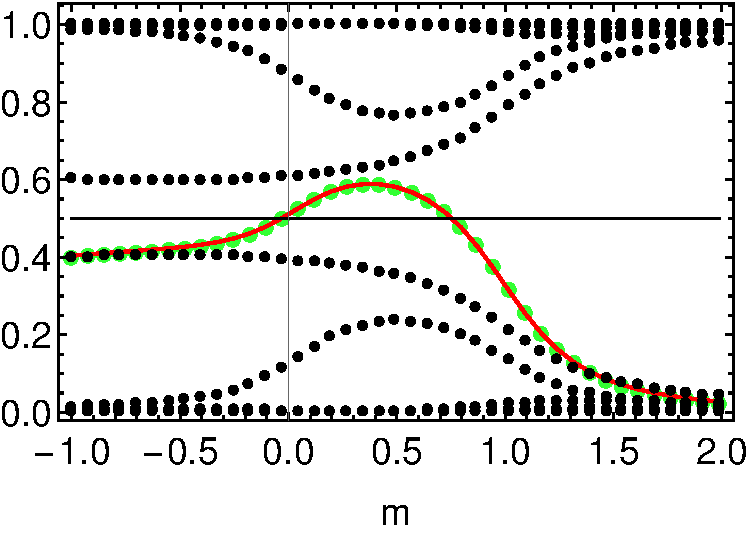
\includegraphics[width=35mm]{2_b.pdf}
}
}
\caption{\mariac{system size?}Entanglement spectrum (black), $\chi$ (green) and $\frac{\gamma}{2\pi}$ (red) for a cut in the phase diagram through the $\nu = 1 \rightarrow \nu = 0$ transition (dashed line in~\ref{fig:bdi_phase_diagram}
	) for $t'=0$ and different values of $\kappa$.}
\label{huang}
\end{figure}

\subsubsection{General case}

In expression~\eqref{eqplusminus} we assigned a `charge'  of $\pm1/2$ to each entanglement eigenstate depending on the eigenvalue ordering, see also appendix~\ref{app:pollmann} and the related discussion in Ref.~\cite{Zaletel2014}. 
In order to generalize this to systems for which the ES is not equidistant  one needs to know how to properly assign this $\pm 1/2$ charge to each entanglement mode. We found that this is done according to their localization. 
We separate the eigenstates of the entanglement Hamiltonian (or alternatively the reduced correlation matrix) into a \emph{right} and \emph{left} set depending on whether $\expval{\hat{X}}_i > L/4$ or $\expval{\hat{X}}_i < L/4$ (region $A$ ranges from $0$ to $L/2$) and we assign the charges $q_r = +1/2$ and $q_l = -1/2$, respectively.
 Expression \eqref{eqplusminus} then generalizes to
\begin{equation}
\chi = \frac{1}{2} \left( \sum_{i\in r}\xi_i-\sum_{i\in l}\xi_i+ N_A \right) \quad {\rm mod} \quad 1.
\label{eq_loc}
\end{equation}

In order for this expression to be well-defined however we need localized eigenstates. 
Non-degenerate eigenstates of the EOS are automatically localized, but degenerate or nearly-degenerate eigenstates (i.e. those exponentially close to $\xi=0,1$) are not necessarily localized. 
It turns out that we need not worry about the latter set of states, because changing their charge from say $1/2$ to $-1/2$ only changes $1/2(\sum_{i\in r} \xi_i - \sum_{i\in l}\xi_i)$ in Eq.~\eqref{eq_loc} by an integer, which is canceled \mariac{better expression?} by mod 1. 
Also in the case where eigenstates are double degenerate we need not worry about localizing them, because computing the expectation value of the position operator will automatically assign the correct number of eigenstates to the left/right half of $A$. 
This is no longer true for four-fold, or higher-fold, degenerate states.
%In Fig.\ref{huang}.a the doubly-degenerate states have contributions from both edges. Performing the above classification will always lead to assigning one state as \emph{left} and the other one as \emph{right} so there is no issue, but this is no longer true for four-fold, or higher, degenerate states. 
%The eigenstates close to $1$ and $0$ are also highly degenerate and thus delocalized over the whole chain. However in this case this is irrelevant since the difference in $\chi$ from changing the charge in one of these modes is either $0$ or $1$, which is cancelled anyway by taking the modulo $1$, so the expression \ref{loceq} is well-defined \carlos{up to exponentially small errors?}.


In order to ensure that we obtain localized entanglement eigenstates,  we diagonalize $C_A + \lambda C_A\hat{X}C_A$ instead of $C_A$.
For the whole system, one way of obtaining localized eigenstates of the full correlation matrix is to diagonalize $C\hat{X}C$, which results in localized Wannier states. 
$C$ commutes with this operator because it is a projector, but this is not necessarily the case for $C_A$ and $C_A\hat{X}C_A$. 
Far from the edges, however, $C_A$ and $C$ are equivalent, so that the states at $\xi=1$ will localize into Wannier states by adding the $\lambda C_A\hat{X}C_A$ term.
The rest of the eigenstates will also localize because this term, as it splits the degeneracies. 
But as it does not commute with $C_A$ close to the virtual edges,  it will modify the eigenstates. 
For that reason $\lambda$ must be a small parameter. \mariac{how to scale $\lambda$ with system size}. 
%\mariac{do not commute 
%	relation to wannier states
%	how to choose lambda }
%where $\lambda$ is a parameter that must be high enough to split all degenerate states into localized ones but small enough to not perturbe the EOS. 

In Fig.\ref{2} we show two examples that highlight the importance of the localization structure of the ES. 
In subfigures (a) and (b), we compute the EOS for varying $m$ at  $t=1$, $t'=2$, indicated by the solid line  in the phase-diagram~\ref{fig:bdi_phase_diagram}, in the presence of two different symmetry breaking terms: (i) $\kappa =0.3$, $\kappa'=0$ and (ii) $\kappa=0$, $\kappa'=0.3$.  
For $\kappa=\kappa'=0$, there is a phase transition $\nu = 2 \rightarrow 0 $ at $m=2$, whereas both choices of symmetry breaking render the system trivial  for all $m$.
However, the two symmetry breaking terms split the four-fold degenerate $\xi=1/2$ midgap states very differently, thus resulting in completely different Zak phases despite the superficial resemblance of their respective EOS.  
While $\kappa'$ splits the four-fold degenerate states into two two-fold degenerate pairs at opposite edges whose contribution cancels, $\kappa$ split them into two $left-left$ and $right-right$ pairs, with a finite contribution to the Zak phase. 
In subfigures (c) and (d), we consider the same symmetry breaking terms, but now for $t=1$ and $t'=-2$, where the BDI systems shows a phase transition  $\nu=2\rightarrow 1\rightarrow 0$. 
Note that the $\kappa'$ term does not render the $\nu=1$ phase trivial, and the Zak phase will remain quantized in that region, see Fig.~\ref{2}(d). 
Also here, Eq.~\ref{eq_loc} correctly reproduces the Zak phase for all values of $m$. 
Note that in all examples shown in this subsection, the observations made in references \cite{Huang2012,Huang2012-2}, i.e. that the behavior of the Zak phase resembles that of the entanglement occupancy midgap states, do not apply anymore. 

\begin{figure}[h!]
	\centering
	\makebox[0pt]{
		\subfloat[$t = 1, t' = 2,$   $\kappa =0.3, \kappa' = 0$]{
			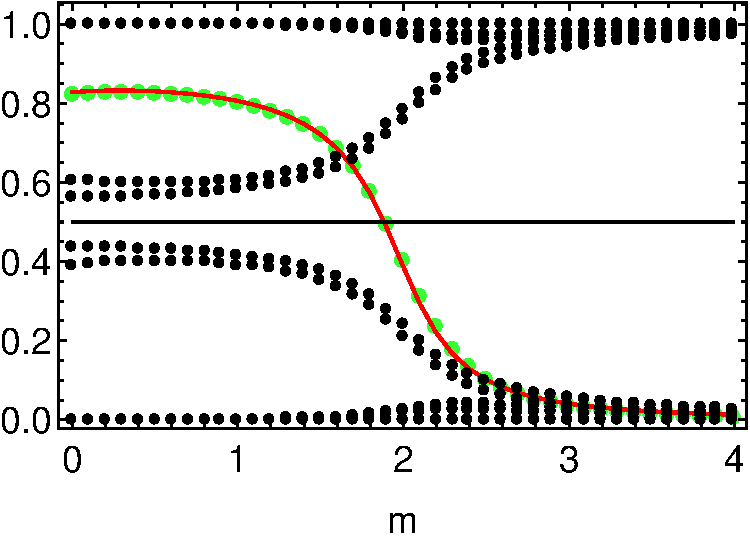
\includegraphics[width=35mm]{3_a.pdf}
		}
		\subfloat[$t = 1, t' = 2,$ $\kappa = 0, \kappa' = 0.3$]{
			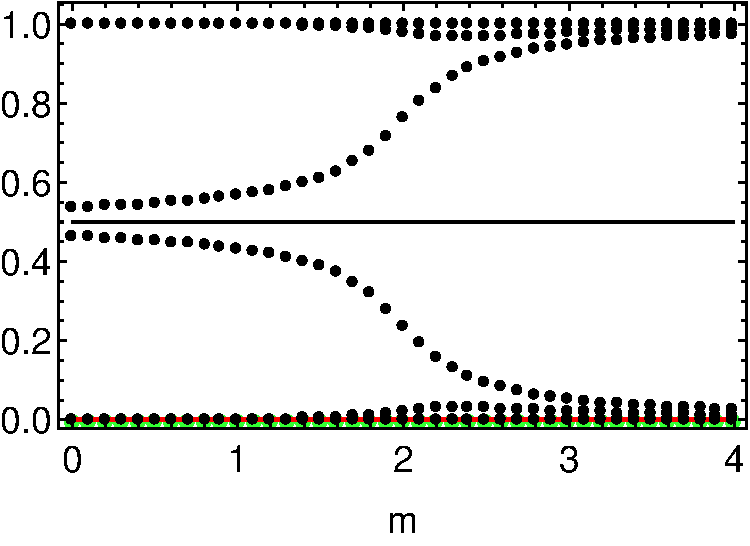
\includegraphics[width=35mm]{3_b.pdf}
		}
	}\hspace{0mm}
	
	\makebox[0pt]{
		\subfloat[$t = 1, t' = -2,$ $\kappa = 0.3, \kappa' = 0$]{
			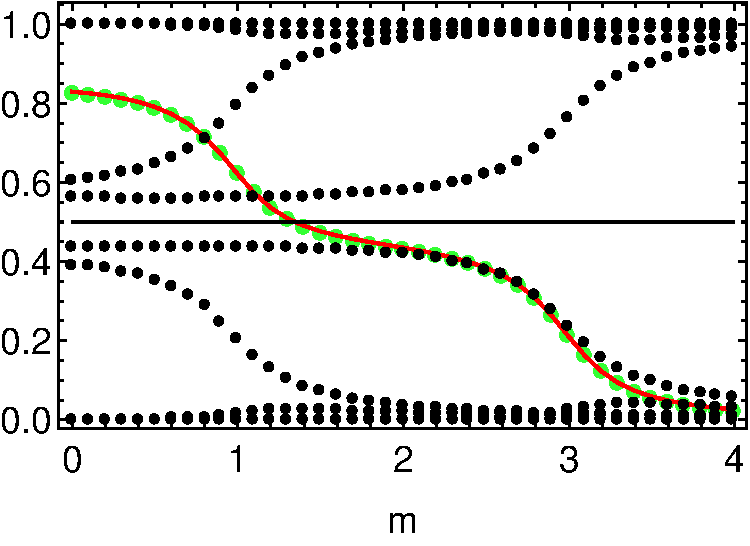
\includegraphics[width=35mm]{3_c.pdf}
		}
		\subfloat[$t = 1, t' = -2,$ $\kappa = 0, \kappa' = 0.3$]{
			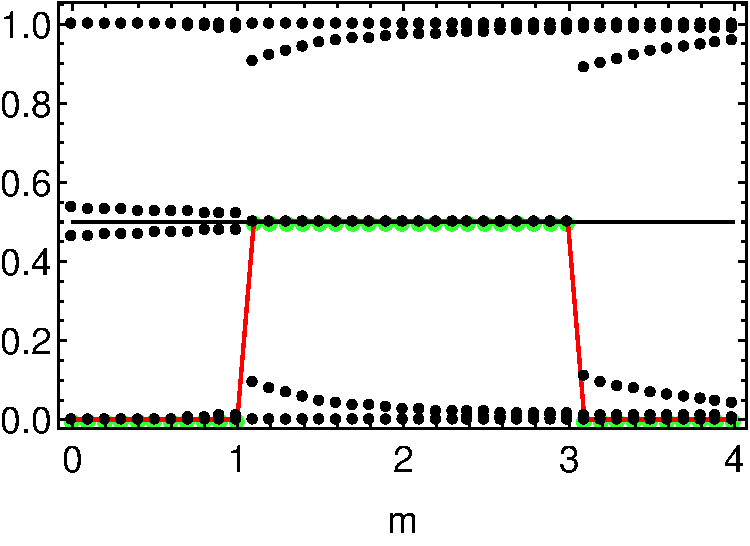
\includegraphics[width=35mm]{3_d.pdf}
		}
	}
	\caption{Entanglement spectrum (black), $\chi$ (green) and $\gamma$ (red) for two different cuts,  continuous line for a,b, and dotted line for c,d plots, Showing a more diverse ES where more than one midgap state is present. }
	\label{2}
\end{figure}

\mariac{issue about  the ambiguity about right - left vs left - right, connect with discussion about Zaletel results and their convention?}
This relation between the Zak phase and the EOS is a consequence of an identity between the Zak phase and the many-body entanglement spectrum previously found for infinite chains \cite{Zaletel2014}. In Appendix A we modified this derivation to account for the periodic boundary conditions we use and show how their result reduces to Eq.~\eqref{eq_loc} when expressing it in terms of the EOS.


Let us also discuss an alternative way of computing Zak phase. 
Using the fact that $N_A = \Tr C_A$, we can rewrite $\chi$ as
\begin{equation}
\chi = \left(\sum_{i\in r} \xi_i\right) \, {\rm mod} \, 1.
\label{eq:chihom}
\end{equation}
A simpler way to compute this quantity is by obtaining $C_A$ for an open chain, labeled as $C_A^{ o}$. 
For a sufficiently long  chain the right eigenvalues will remain the same, %as we still place a virtual cut in the middle of the chain 
but the left eigenvalues will no longer be present. 
This allows one to simply compute
\begin{equation}
\chi = \Tr C_A^{o} \, {\rm mod} \, 1.
\end{equation}
This method, however, will introduce a stronger finite size effect and requires substantially larger systems for the same accuracy. 
In addition, it only works for homogeneous systems as explained below. 


Before proceeding with the inhomogeneous systems, let us explain why the expression~\eqref{eqplusminus} simplifies so much for systems with an equidistant ES. 
First note that for translation invariant systems, the ES of the right and the left edge are related by an overall '-' sign, i.e. for each eigenvalue $\epsilon$ on the right edge, there is a corresponding value $-\epsilon$ on the left edge. 
Since the spectra are equidistant, this implies that the two edge spectra are merely shifted with respect to each other.
Note that  the shift could be zero, e.g.  in presence of a symmetry. 
Independent of the shift, the simple assignment of $ (...+-+-+-...)$ will automatically assign charges $\pm 1/2$ to each edge. 
The only remaining issue is whether this simple recipe assigns charge $+1/2$ or $-1/2$ to the right edge.
In presence of a symmetry, this question is irrelevant \mariac{better expression?} because of the degeneracy. 
In general, it implies that $\chi$ as defined in Eq.~\eqref{eqplusminus} only gives the Zak phase up to an overall sign. 
This issue can be fixed by determining the localization of a single eigenstate. 

%The reason is that, unless they are degenerate, the ordered eigenstates always come with alternating edge localization (...left-right-left-right...)\mariac{ref to peschel}, so that the signs assigned are always . 
%\mariac{expand}
%\mariac{issue about crossing spectra?}
%If the eigenvalues cross each other this only adds a global minus sign, however this unlikely and usually only happens when all eigenvalues are close to $0$ and $1$ and $\chi$ is therefore small. 


% - % - % - % - % - % - % - % - % - % - % - % - % - % - % - % - % - % - % - % - % - % - % - % - % - % - % - % - % - % - % - % - % - % - % - % - % - % 

\section{Inhomogeneous systems}

In reference \cite{Zaletel2014} translational invariance was used to derive the relation between the many-body entanglement spectrum and the Zak phase. If this symmetry is broken by adding, for example, weak disorder, this result is no longer true. However we found, as our main result, that one can still obtain the Zak phase as the cut-average of the relation derived for homogeneous systems. For some systems this can be written as (\carlos{not sure about this phrasing})
\begin{align}
\bar{\chi} =\left(\frac{1}{L}\sum_{s=1}^L (\chi_s \, \rm{mod} \, 1)\right)\, \rm{mod} \, 1,
\label{eq:inh_simple}
\end{align}
where
\begin{equation}
\chi_s = \frac{1}{2} \left( \sum_{i\in r}\xi^s_i-\sum_{i\in l}\xi^s_i  + N_A \right)
\end{equation}
is obtained for cuts at sites $s$ and $s+L/2$. In Fig.\ref{fig:simple_inh}.b we show the same system as in Fig.\ref{2}.c with an added moderate disorder in the $\kappa$ parameter shown in \ref{fig:simple_inh}.a . We show the EOS of one cut with that particular $\chi_s$, which differs from the Zak phase. The Zak phase is shown to be recovered by the cut-average of $\chi$. Next we show the results for the same system with $m=-2$, and a continuous profile for $\kappa$ shown in \ref{fig:simple_inh}.c. In Fig. \ref{fig:simple_inh}.d is shown how the EOS and $\chi_s$ depends on the cuts, and how the Zak phase is again recovered by the cut-averaged $\chi$.

\begin{figure}[h!]
\centering
\makebox[0pt]{
\subfloat[$\kappa_i$]{
  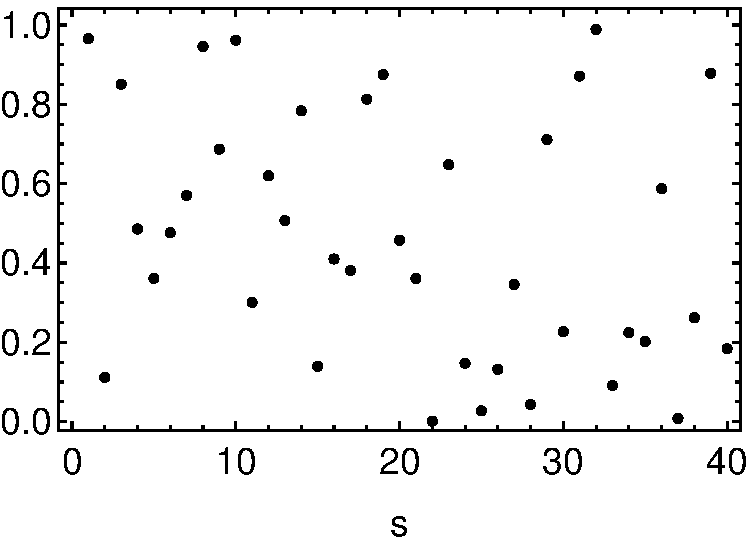
\includegraphics[width=35mm]{4cdisorderkap.pdf}
}
\subfloat[$t=1,t'=-2,s=0$]{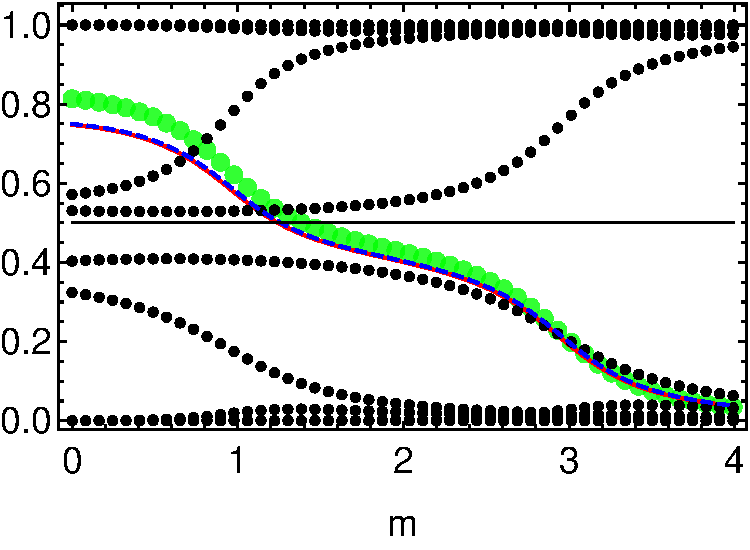
\includegraphics[width=35mm]{4cdisorderES.pdf}
}
}\hspace{0mm}

\makebox[0pt]{
\subfloat[$\kappa_i$]{
  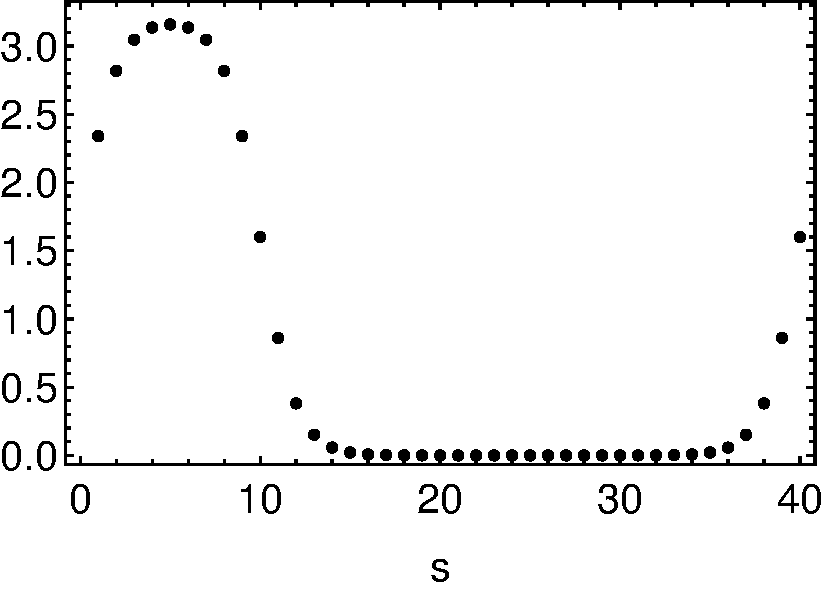
\includegraphics[width=35mm]{simplecutkap.pdf}
}
\subfloat[$t=1,t'=-2,m=2$]{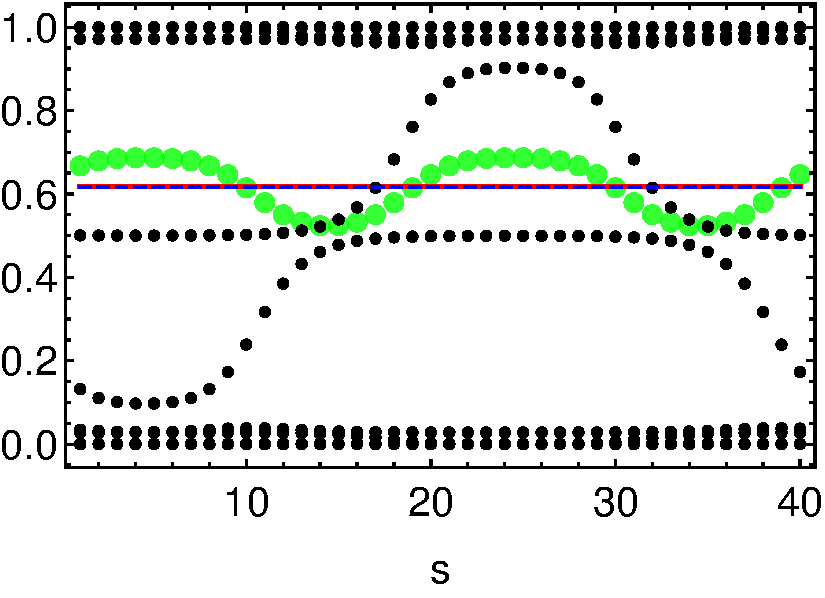
\includegraphics[width=35mm]{simplecutES.pdf}
}
}\hspace{0mm}

\makebox[0pt]{
\subfloat[$\kappa_i$]{
  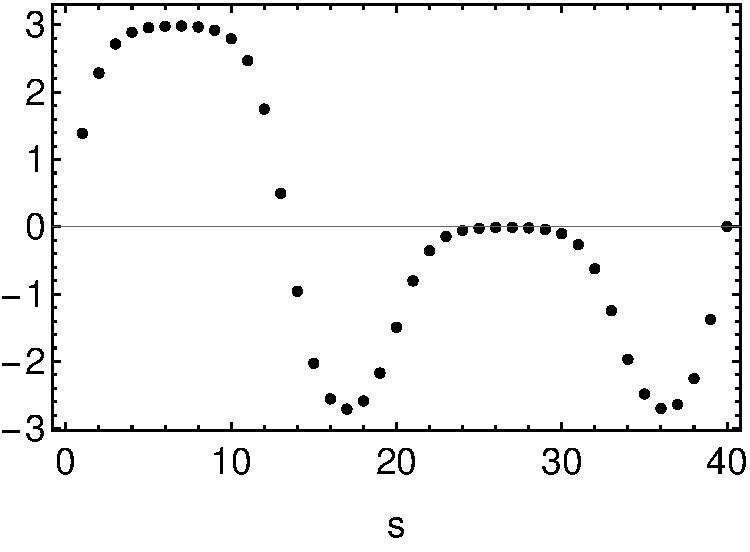
\includegraphics[width=35mm]{simplecutavgaround0kap.pdf}
}
\subfloat[$t=1,t'=-2,m=1$]{\includegraphics[width=35mm]{simplecutavgaround0.pdf}
}
}
\caption{In a) and b) we show the system in Fig. 4.c with an added disorder. we show the ES (black) and $ \chi_s \, {\rm mod} \, 1$ (green) for one particular cut,$\gamma$ (red) and $\expval{\chi_s}_{\rm cuts}$ (blue dashed). In c) and d) we show the same system at $m=2$ and a continuous homogeneous profile for $\kappa_i$. In e) and f) we show a case where using \eqref{eq:inh_simple} fails. We show the ES and $\chi_s$ for all cuts. }
\label{fig:simple_inh}
\end{figure}

We have shown two cases were using expression \ref{eq:inh_simple} leads to the correct result, but this is in fact not the general case, as we can see in Fig.\ref{fig:simple_inh}.f . The average of a circular quantity is not uniquely defined and the choice we made in Eq.\ref{eq:inh_simple}, which equates to averaging the values in $(0,1)$ around $1/2$ (\carlos{is this clear?}) turns out to work in certain cases. How to perform this circular average is a priory not known, we can only judge after we compute the Zak phase independetly if we used the correct choice or not. Therefore in order to proceed we need to get rid of the circular average which leaves us with
\begin{align}
\bar{\chi} =\left(\frac{1}{L}\sum_{s=1}^L \chi_s \right)\, \rm{mod} \, 1,
\label{eq:inh_fixed}
\end{align}
but this however has to be done carefully. So far we have naively separated our eigenstates into \emph{left} and \emph{rigth} sectors, assigned the charges acordingly, and took the modulo 1 to eliminate the contribution of the bulk modes that localize at the center of A. The problem resides in the classification of these bulk modes. Even if the rest of the EOS remains constant, due to the inhomogeneity a bulk mode can cross the middle of region A, as shown in Fig.\ref{fig:loc_fix}, which will change $\chi$ by $1/L$, even though choosing $L/4$ as the separation between the \emph{left} and \emph{rigth} sectors is not physical. In order for \ref{eq:inh_fixed} to work properly the contribution from the bulk modes, which should vanish in the end, must remain constant across the different cuts. In order to achieve this we have to choose a cut-dependent threshold that the bulk modes do not cross. We choose this threshold, $l_s$, as the mean position of two of the eigenstates close to this middle point of A, as shown in Fig.\ref{fig:loc_fix}. This is done in practice using the Wannier states (\carlos{Do I explain exactly how do I do it numerically?}).
Note that in the thermodynamic limit it does not matter if the position of these eigenstates cross as they are degenerate, the only important thing is that the number of bulk modes at each sector remains constant (\carlos{Not sure about this phrasing either}). 

The reason Eq.\ref{eq:inh_simple} works in some cases is that if, assuming the correct constant bulk contribution, $\chi_s \in [n,n+1)$, wher $n$ is an integer, then taking the modulo 1 before or after averaging does not affect the final result. The same argument can be generalize for a $\chi_s \in [a+a,1)$, for any real $a$, given that we offset the modulo 1 in Eq.\ref{eq:inh_simple} appropiately.


\begin{figure}[h!]
\centering
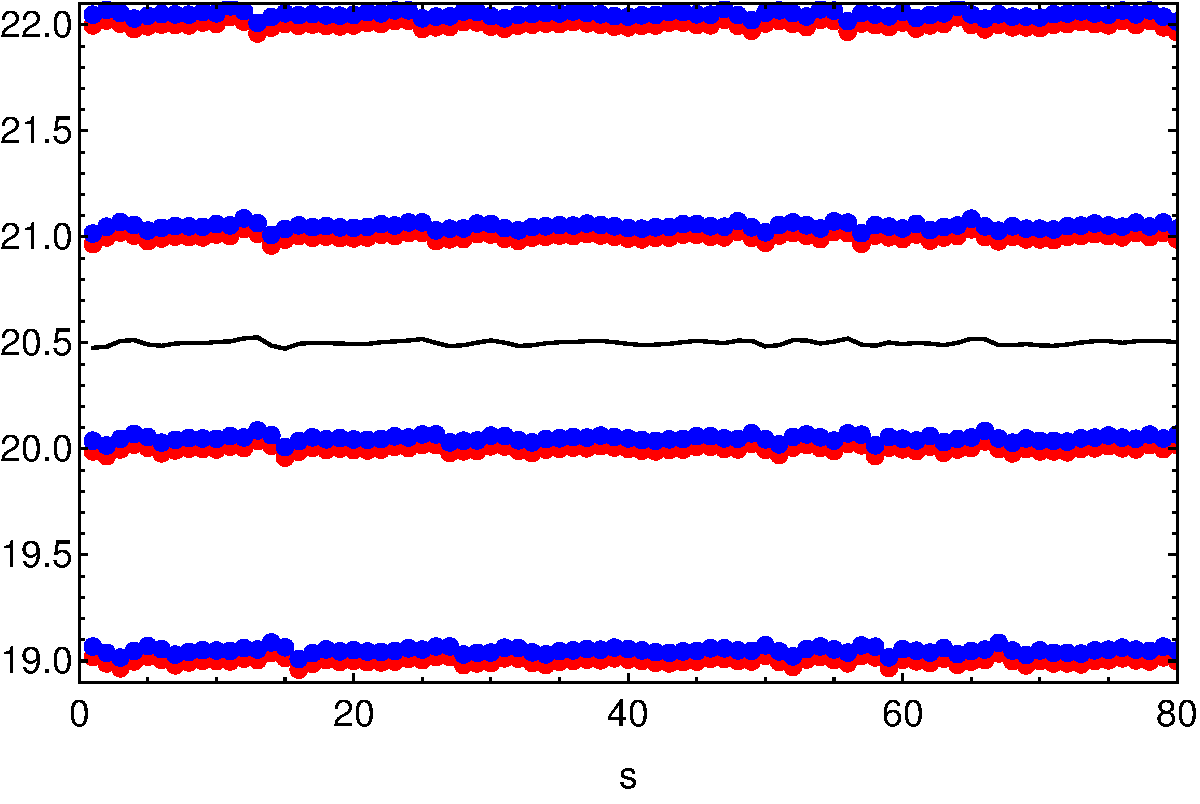
\includegraphics[width=70mm]{loc_fix.pdf}
\caption{Average position of the Wannier states in red and, slightly shifted, the localized entanglement eigenstates 
in blue. In black we show the threshold $l_s$ obtained as the mean value of the two Wannier states close de $19$ and $20$) $L=80,\lambda=10^{-6}, t = 1, t'= 2, m=0$}
\label{fig:loc_fix}
\end{figure}




As the sign assigned to the bulk modes becomes relevant in the inhomogeneous case one might think that it is better to use the open chain, $\chi_s = \Tr C_A^{{\rm open},s}$, as one avoids the issue of having to assign any signs at all. Although this is true we find another problem. By adiabatically tuning down the coupling between the $L$ and $1$ sites we see that the eigenvalues of the $left$ modes flow to either $0$ or $1$. This can lead to discontinuities in the number of bulk modes at $\xi=1$ which again result in an incorrect cut-average. \carlos{Do we want to include is? Or leave it for later?}


% - % - % - % - % - % - % - % - % - % - % - % - % - % - % - % - % - % - % - % - % - % - % - % - % - % - % - % - % - % - % - % - % - % - % - % - % - % 

\section{Superconducting systems}

However, as we did for systems without translational invariance, one can extend this identity for systems with pairing terms as well. Since one computes the Zak phase from the single-particle Bogoliubov-de Gennes Hamiltonian, we can obtain the correspondent ES and everything discussed above should apply as well. Take for example the kitaev chain, with the following Hamiltonian
\begin{align*}
H =& -\mu \sum_{i} c_i^\dagger c_i - t \sum_{i}\left( c_{i+1}^\dagger c_i + {\rm h.c.}\right) \\
&+  \sum_{i}\left( \Delta c_{i} c_{i+1} + {\rm h.c.}\right).
\end{align*}
Using the spinor $\phi_i^\dagger = (c_i^\dagger, c_i)$, we can rewrite the Hamiltonian as
\begin{align*}
&H = \frac{1}{2}\sum_i \phi^\dagger_i H_{BdG,ij} \phi_j,\\
&H_{BdG,ij} = -\mu \tau_z \delta_{ij} - (t \tau_z + i\Delta \tau_y )\delta_{i,j+1}- (t \tau_z - i\Delta \tau_y)\delta_{i,j-1}.
\end{align*}
Note that by taking $t' = \kappa = \kappa = 0$ in the BDI model, Eq. \ref{bdi_model}, we obtain
\begin{align*}
H_{ij} =& m \sigma_x\delta_{ij} + \frac{1}{2} t \left[(\sigma_x + i \sigma_y)\delta_{i,j+1} + (\sigma_x - i \sigma_y) \delta_{i,j-1} \right],
\end{align*}
which is just the Bogoliubov-de Gennes Hamiltonian of the Kitaev chain by rotating $x$ into $z$ and identifying $\mu = -m, t_{\rm Kit} = -t_{BDI}/2, \Delta = -t_{BDI}/2 $. From Fig.\ref{bdi_phase_diagram} we see that the $BDI$ model transitions from $\nu = 1$ to the trivial phase at $t=0, m=\pm t_{BDI}$, or alternatively, when $\mu = \pm 2 t_{Kit}$, which is the known result for the Kitaev chain. Therefore the results already shown for the BDI model studied here are also applicable to the Kitaev chain.  

\section{Conclusion}

It was previously known that the Zak phase was encoded in the many-body entanglement spectrum. Here we have shown how it is encoded in the single-body entanglement spectrum. This relation is simpler than the one involving the MBES and it provides more insight into the ES. We have furthermore shown how this relation generalizes to inhomogeneous and superconducting systems, where it was not previously shown to be present. Our result also provides a new way of computing the Zak phase for inhomogeneous systems where instead of diagonalizing a $2L\times 2L$ matrix one has to diagonalize $L$ matrices of size $L\times L$, which in some cases might be computationally favorable. (\carlos{can we get insight on this?}). 

\bibliography{references}	

	
\appendix

% - % - % - % - % - % - % - % - % - % - % - % - % - % - % - % - % - % - % - % - % - % - % - % - % - % - % - % - % - % - % - % - % - % - % - % - % - % 

\section{Computing the Zak phase from the Schmidt decomposition}\label{app:pollmann}
\maria{In this appendix, we review  how to compute the Zak phase from the Schmidt decomposition~\cite{Zaletel2014}and relate it to our own results of Eq.s~\eqref{eqplusminus} and \eqref{eq_loc}.}

\mariac{notation ES/EOS consistent with main text?}

\mariac{add some explanatory sentences?}

Consider a chain with periodic boundary conditions. A Schmidt decomposition for two bipartite cuts gives the ground state
\begin{equation}
\ket{\psi} = \sum_{p,q} \ket{p,q}_A s_p \ket{p,q}_B s_q,
\end{equation}
where we assume that the size of each subsystem is big enough so that the cuts can be considered independent of each other. We can now take subsystem B and glue its ends together to obtain the ground state of a ring with a single cut. If we include a flux threading inside the ring we obtain
\begin{equation}
\ket{\psi^\phi} = \sum_p s_p \ket{p,p}_B e^{i\phi Q_p},
\end{equation}
The many-body states $\ket{p,p}_B$ can be built by occupying the different ES eigenstates and are therefore characterized by a set of occupying numbers $\{n\}_p$. The many-body entanglement spectrum can also be expressed in terms of the single-particle one \cite{Alexandrinata2011} as
\begin{align}
s_p^2 =& \prod_{i \in {\rm occ}} \xi_i \prod_{i \in {\rm empty}}(1-\xi_i) \\
=& \prod_i (1-\xi_i)\left(\frac{\xi_i}{1-\xi_i} \right)^{n_i}
\end{align}
And the charge can be assigned so that $Q_p = \sum_{\alpha = l,r} q_\alpha\sum_{i \in \alpha} n_i$ with the constrain that $q_r= q_l-1$ \textcolor{red}{Why?}. As the main result of \cite{Zaletel2014} the Zak phase is then found to be
\begin{align}
e^{i\gamma} = e^{2\pi i \sum_p s_p^2 Q_p}  \bra{\psi^0}\ket{\psi^{2\pi}},
\label{zaletel}
\end{align}
where the monodromy is given by
\begin{align}
\bra{\psi^0}\ket{\psi^{2\pi}} =& \sum_p s_p^2 e^{2\pi i Q_p}.
\end{align}
Consider the exponential term
\begin{align*}
e^{2\pi i (q_L N^p_l + (1-q_l)(N^p_r+N^p_b))} =& e^{2\pi i (q_l N^p_l + (1-q_l)(N-N^p_l))} \\
=& e^{4\pi i q_l N^p_l}e^{2 \pi i (N-N^p_l)}e^{-2\pi i q_l N },
\end{align*}
where $N^p_\alpha = \sum_{i \in \alpha} n_i$ and the total number of electrons, $N = \sum_{\alpha = b,l,r} N^p_\alpha$, is independent of $p$. We will consider two natural choices, $q_l = 1,1/2$, for which we have
\begin{align}
\bra{\psi^0}\ket{\psi^{2\pi}} =& 
\begin{cases}
1 & \text{for} \quad q_l = 1 \\
e^{N\pi i} & \text{for} \quad q_l = 1/2,
\end{cases}
\end{align}
where we used that $\sum_p s_p^2 = 1$. The change in the monodromy between both choices is accompanied by a change in the exponential term in Eq.\ref{zaletel}, so that both charge choices are equivalent.

Expressing the contribution of the many-body entanglement spectrum to the Zak phase in terms of the ES, we have
\begin{align*}
\gamma' = 2\pi \sum_{n_i = 0,1} \left(\sum_{i } n_i q_i\right) \left(\prod_m (1- \xi_m)\left(\frac{\xi_m}{1-\xi_m} \right)^{n_m} \right) ,
\end{align*} 
Consider now its derivative with respect to a particular entanglement eigenvalue
\begin{align}
\frac{1}{2\pi}\frac{\partial \gamma'}{\partial \xi_p} =& \sum_{\{n_k\}=0,1}\left(\sum_{i } n_i q_i\right)\frac{n_p - \xi_p}{\xi_p^{1-n_p}(1-\xi_p)^{n_p}}\\
&\times \left(\prod_{m\neq p} (1- \xi_m)\left(\frac{\xi_m}{1-\xi_m} \right)^{n_m} \right)
\end{align}
where
\begin{equation}
 \frac{n_p - \xi_p}{\xi_p^{1-n_p}(1-\xi_p)^{n_p}} = 
  \begin{cases}
    -1, & \text{for } n_p=0 \\
    1, & \text{for } n_p = 1 \\
  \end{cases}	
\end{equation}
Therefore we have
\begin{align*}
\frac{1}{2\pi}\frac{\partial \gamma'}{\partial \xi_p} =& -\sum_{\substack{\{n_{k\neq p}\}=0,1 \\ n_p = 0}}\left(\sum_{i \neq p} n_i q_i\right)\prod_{m\neq p} (1-\xi_m)\left( \frac{\xi_m}{1-\xi_m} \right)^{n_m} \\
&+ \sum_{\substack{\{n_{k\neq p}\}=0,1 \\ n_p = 1}}\left(\sum_{i \neq p} n_i q_i +q_p\right) \prod_{m\neq p} (1-\xi_m)\left( \frac{\xi_m}{1-\xi_m} \right)^{n_m} \\
=&q_p\sum_{\{n_{k\neq p}\}=0,1} \prod_{k\neq p} (1-\xi_k)\left( \frac{\xi_k}{1-\xi_k} \right)^{n_k} \\
\end{align*}
Expand now the sum  for another occupation number $n_{p'} = 0,1$ 
\begin{align*}
\frac{1}{2\pi}\frac{\partial \gamma'}{\partial \xi_p} =& q_p\sum_{\substack{n_{k \neq p \neq p'}=0,1\\ n_{p'}= 0}} (1-\xi_{p'})\prod_{k\neq p,p'} (1-\xi_k)\left( \frac{\xi_k}{1-\xi_k} \right)^{n_k} \\
&+ q_p\sum_{\substack{n_{k \neq p \neq p'}=0,1\\ n_{p'}= 1}} \xi_{p'}\prod_{k\neq p,p'} (1-\xi_k)\left( \frac{\xi_k}{1-\xi_k} \right)^{n_k} \\
 &=q_p\sum_{\substack{n_{k \neq p \neq p'}=0,1}} \prod_{k\neq p,p'} (1-\xi_k)\left( \frac{\xi_k}{1-\xi_k} \right)^{n_k} 
\end{align*}
doing this for the rest of the occupation numbers we obtain 
\begin{equation}
\frac{1}{2\pi}\frac{\partial \gamma'}{\partial \xi_p} = q_p,
\end{equation}
so that 
\begin{align*}
\gamma =& \gamma' - i\log(\bra{\psi^0}\ket{\psi^{2\pi}})\\
=& \sum_{i}q_i \xi_i - i\log(\bra{\psi^0}\ket{\psi^{2\pi}})\\
\end{align*}
and we have recovered equation \ref{mainl}. 

\section{Alternative expression for the correlation matrix}\label{app:CM}
In this appendix, we show how to express the correlation matrix in terms of the Hamiltonian, used in Eq.~\eqref{eq:corr_mat2}. 
We consider the generic, quadratic Hamiltonian in one dimension of Eq.~\ref{eq:quadr_Ham}, which is diagonalized by a unitary matrix $U$ with 
	\begin{align}\label{eq:D}
	H&=UDU^\dagger& \mbox{with } D=\mbox{diag}(E_{p\mu}).
	\end{align} 
In terms of the fermionic operators that diagonalize the Hamiltonian, 
\begin{align}
& \gamma_{i\alpha} = \sum_{j\beta}u_{j\beta}^{i\alpha \, \ast} c_{j\beta},
%& c_{i\alpha} = \sum_{j\beta} u^{j\beta}_{i\alpha} \gamma_{j\beta}
\end{align}
we find that the correlation matrix can be written as 
\begin{align}\label{eq:corr_mat}
C_{ij}^{\alpha \beta} =& \sum_{pq,\mu\nu} u^{q\nu }_{j\beta} u^{p\mu \, \ast}_{i\alpha} \expval{\gamma^\dagger_{p\mu} \gamma_{q\nu} }\nonumber \\
=&  \sum_{p\mu} u^{p\mu }_{j\beta} u^{p\mu \, \ast}_{i\alpha} \expval{\gamma^\dagger_{p\mu} \gamma_{p\mu} }\nonumber \\
=&  \sum_{p\mu} u^{p\mu }_{j\beta} u^{p\mu \, \ast}_{i\alpha} [1-{\rm sign}(E_{p\mu})]/2.
\end{align}
The first term of the last line is simply a kronecker delta between both sets of indices. 

The second term can be rewritten, using Eq.~\ref{eq:D}, as
\begin{align}
UD(\abs{D})^{-1}U^\dagger =& UDU^\dagger U(D^2)^{-1/2}U^\dagger
\end{align}
We can rewrite this expression further by noting that 
\begin{align}
[U (D^2)^{-1/2} U^\dagger]^2 =& U (D^2)^{-1/2} U^\dagger U  (D^2)^{-1/2} U^\dagger \nonumber\\
=&  U (D^2)^{-1/2}  (D^2)^{-1/2} U^\dagger \nonumber\\
=&  U (D^2)^{-1} U^\dagger \nonumber\\
=&  (U D^2 U^\dagger)^{-1}.
\end{align}
Therefore,
\begin{align*}
U (D^2)^{-1/2} U^\dagger =&(U D^2 U^\dagger)^{-1/2} 
\end{align*}
and we conclude that
\begin{align}\label{eq:UDDU}
UD(\abs{D})^{-1}U^\dagger =& UDU^\dagger(U D^2 U^\dagger)^{-1/2} \nonumber\\ 
=& H(H^2)^{-1/2}.
\end{align}
Combining Eq.s~\eqref{eq:corr_mat},  and \eqref{eq:UDDU}, we arrive at the final expression of the correlation matrix in Eq.~\eqref{eq:corr_mat2}. 


\section{$\lambda$ term}


In order to ensure that we obtain localized entanglement eigenstates,  we diagonalize $C_A^\lambda = C_A + \lambda/L^2 C_A\hat{X}C_A$ instead of $C_A$, where $\lambda$ is our small parameter and the reason we include the $L^2$ scaling will be explained below.
For the whole system one way of obtaining localized eigenstates of the full correlation function (\carlos{also the Hamiltonian?}) is to diagonalize $C\hat{X}C$, which results in localized Wannier states. $C$ commutes with this operator because it is a projector, but this is no longer the case for $C_A$. Far from the edges however, $C_A$ and $C$ are equivalent, so that the states close to $\xi=1$ will perfectly localize into Wannier states by adding the $\lambda$ term. Note that in the thermodynamic limit the operator $\hat{X}$ acts as proportional to an identity for localized states. Therefore in this limit the localized eigenstates of $C_A$ far from $\xi = 0,1$ are also eigenstates of $C_A^\lambda$ while their mixture is not. Threfore this operator breaks all degeneracies of $C_A$ and results in localized eigenstates.

One has to be careful when choosing the correct $\lambda$. A parameter $\lambda$ which is too small will fail to break the degeneracies and localize the eigenstates. On the other hand the $\lambda$ term will  modify the eigenvalues and introduce an additional error to $\chi$. Assuming localized eigenstates we have $\expval{\hat{X}}_{i\alpha} \simeq i$. Therefore the error it introduces in $\chi$ is roughly
\begin{equation}
\frac{\lambda}{L^2} \sum_{\alpha=1,2}\left( \sum_{i=L/4+1}^{L/2}i-\sum_{i=1}^{L/4}i \right) = \frac{\lambda }{8},
\end{equation}
it is proportional to $\lambda$ and independent on system size. In Fig.\ref{lambdaL} we show this error in $\chi$ together with the maximum width of the eigenstates in the top half of the spectrum (\carlos{as we only care about the midgap states and the bulk modes at 1}), for different system sizes. We see that indeed the error remains constant with system size. In this case most of the bulk modes are above $\xi = 1-10^{-10}$, so that the error coming from the $\lambda$ term is bigger than the one we make by failing to localize the bulk modes. However, by looking at the maximum width of the eigenstates we see three different regions. One region at low system size where the width increases linearly. A second region where the system localizes and the width seems constant, and finally for large systems a third region where the width increases again because the $\lambda$ term is too small to break the degeneracies and localize the eigenstates.


\begin{figure*}[h!]
\centering
\makebox[0pt]{
\subfloat[${\rm Log}_{10}(\chi - \gamma)$ (\carlos{There are errors at $-5,-9,-12$ because that's the order of the eigenvalue of the bulk modes that should cancel pairwise but dont due to failure of localization. Furthermore, the error in yellow around $L=150$ is due to a mode close  to $\xi = 0$ so that it does not appear in Fig. b.})]{
  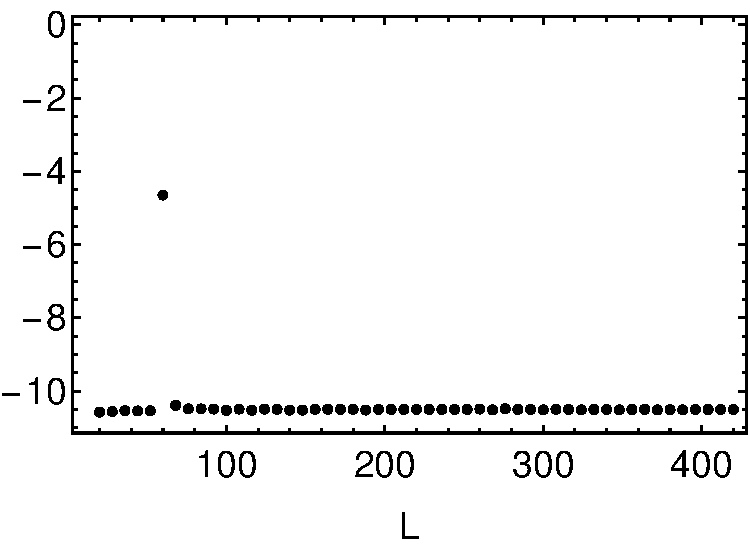
\includegraphics[width=55mm]{lambdaL1.pdf}
}
\subfloat[${\rm Max}\bra{\psi_i}\sigma_x\ket{\psi_i}$ for $\xi_i >1/2$. \carlos{I don't know why the green line localizes so bad. I have to look further into it}]{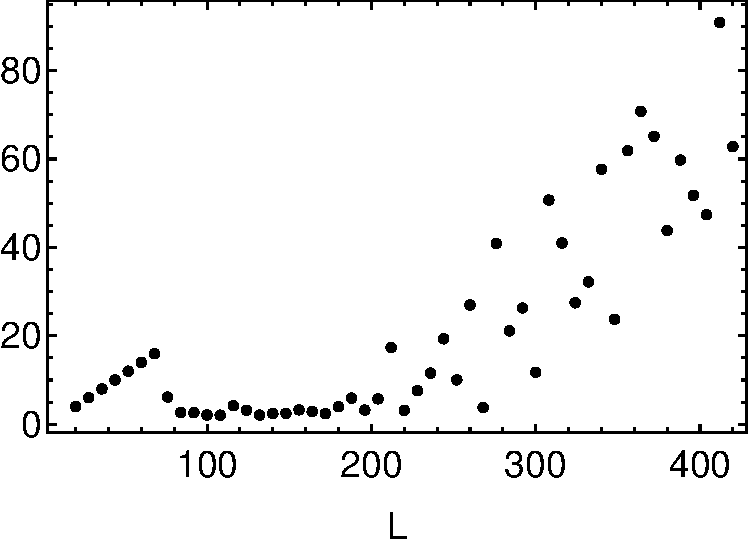
\includegraphics[width=55mm]{lambdaL2.pdf}
}
}
\caption{$t = 1, t'= 2, m=0$ for $-{\rm Log}_{10}[\lambda] = 4,5,6,7,8,9,10$.}
\label{lambdaL}
\end{figure*}

In Fig.\ref{linearRegion} we take a closer look into the first region with a maximum width proportional to the system size. What happens in this region is that due to finite size the midgap modes that localize in the edges overlap so the resulting eigenstates are not localized and are split from $\xi = 1/2$. The boundary where this region ends changes with $\lambda$ and coincides with the point where the splitting from the $\lambda$ term is bigger than the splitting due to finite size. The gap between these midgap modes that mix starts decreasing with larger system size up to a point, where the system starts to localize, where this splitting is roughly constant with system size and proportional to $\lambda$. In the $\nu = 1$ region the two midgap states are degenerate and we do not observe this first linear region, the eigenstates localize for any finite $\lambda$.


\begin{figure*}[h!]
\centering
\makebox[0pt]{
\subfloat[Width of the eigenstate closest to $\xi=1/2$]{
  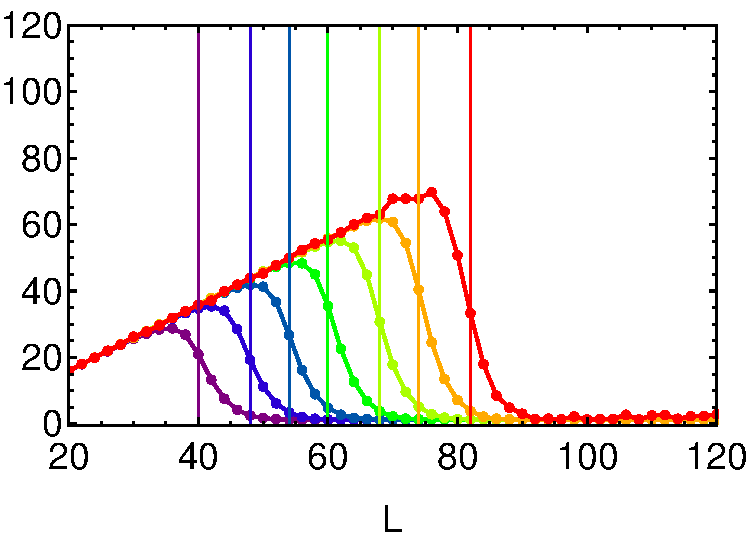
\includegraphics[width=55mm]{linearBoundary.pdf}
}
\subfloat[Gap between the two eigenstates closest to $\xi = 1/2$]{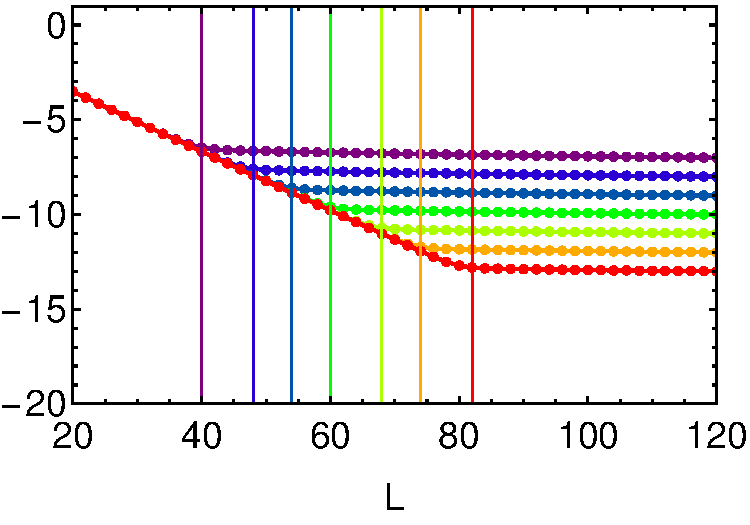
\includegraphics[width=55mm]{linearBoundarysplit.pdf}
}
}
\caption{$t = 1, t'= 2, m=0, \nu=0 , -{\rm Log}_{10}[\gamma] = 4,5,6,7,8,9,10$ for the different colors. Vertical lines are addded to better show how the features of both plots match.}
\label{linearRegion}
\end{figure*}



For inhomogeneous systems the story is slightly different. Due to the cut-average a wrong assignment of the bulk modes leads to an error of order $\mathcal{O}(1/L)$. In Fig. \ref{lambdainh} we have the error made in $\chi$ and the maximum width of the eigenstates for different values of system size $L$. The disorder does not change anything discussed above and we observe the same behavior in the localization as in the homogeneous case.


\begin{figure*}[h!]
\centering
\makebox[0pt]{
\subfloat[${\rm Log}_{10}(\chi - \gamma)$ ]{
  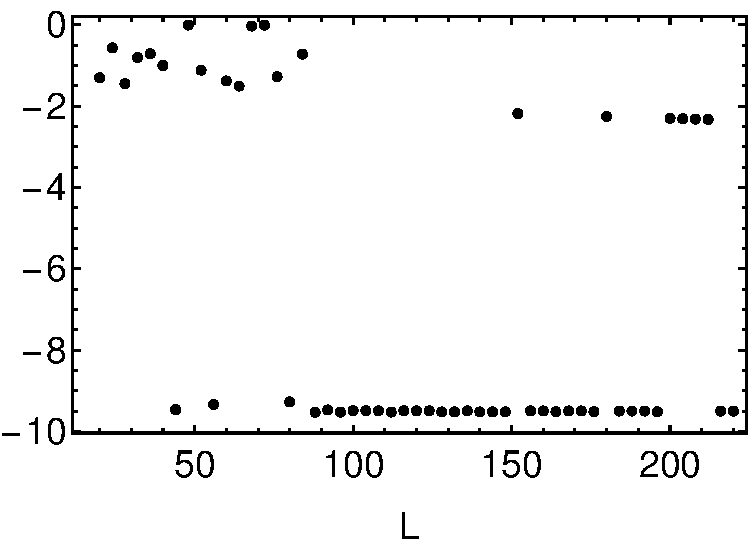
\includegraphics[width=55mm]{lambdaLinherr.pdf}
}
\subfloat[${\rm Max}\bra{\psi_i}\sigma_x\ket{\psi_i}$ for $\xi_i >1/2$.]{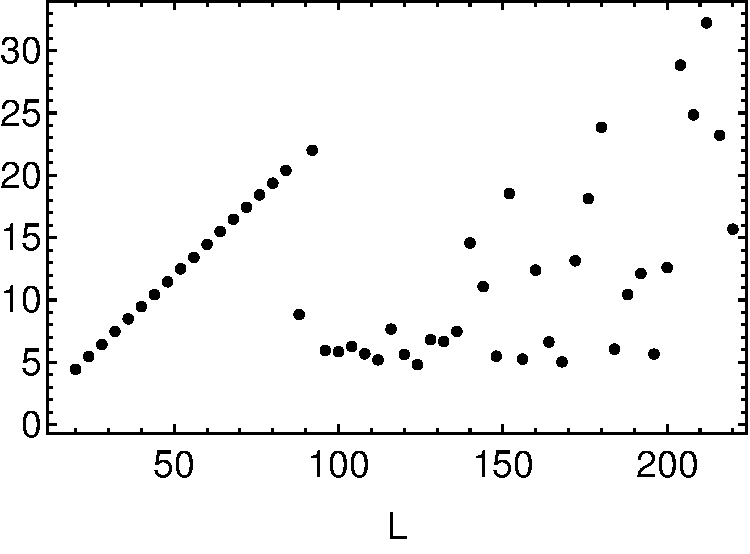
\includegraphics[width=55mm]{lambdaLinhloc.pdf}
}
}
\caption{$t = 1, t'= 2, m=0, \nu=2$. }
\label{lambdainh}
\end{figure*}


\end{document}